\subsection{Nudged Elastic Band}
\label{sec:neb}

\figmiss{NEB force diagram}

\figmiss{Initial and final paths on a PES}

Finding Steepest Decent Paths (SDPs) from a given point is simple by following the gradient with a small step size.
On the other hand, finding specific SDPs that end at minima is not.
The Nudged Elastic Band (NEB) algorithm is concerned with aligning a path with certain SDP paths, the MEP, leading to two minima from a common \sap{1}.

\begin{figure}[t]
  \begin{center}
    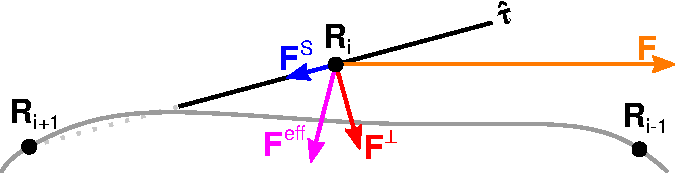
\includegraphics[width=0.6\linewidth]{neb-force-overview}
\parbox{0.85\linewidth}{\caption{An overview schematic of the force components acting within the NEB method.
%$\vR_\text{A}$ and $\vR_0$ are the positions of the dimer images with the greyed out $\vR_\text{B}$ as the virtual image (see \fref{eq:dimer-point-extrapolate}).
%Each force component is labeled with super- and subscripts as follow:
%$0$, $\text{A}$ and $\text{B}$ in subscripts refer to at which point they are calculated,
%$\perp$ and $\parallel$ in superscripts refer to the specific component of the full force (perpendicular and parallel to the minimum mode estimate, respectively),
%$\text{t}$ in a superscript refers to the transformed force (\fref{eq:dimer-transform}),
%$\circlearrowright$ refers to the rotational force (\fref{eq:rotational-force}) and no superscript refers to the PES force.
%$\Dsep$ is the distance between dimer points (\fref{eq:dimer-separation} and $\uvn$ is the current minimum mode estimate.
}}
    \label{fig:neb-force-overview}
  \end{center}
\end{figure}

An initial guess of the path is commonly a, discretisised, linear interpolation bewteen the minima but any guess is suitable as long as the force can be calculated.
Each of the discretisation points is referred to as an image and is simply a replica of the system in question but with different coordinates from the other images.
Each image, $i$, feels two separate forces.
First there is the PES force.
However, only the component perpendicular to the path is retained,
\beq{neb-real-force}
\vF_i^\perp = \vF_i - (\vF_i \cdot \uvt_i) \uvt_i,
\eeq
where $\uvt$ is the tangent to the path.
Second, there is a force acting purely along the tangent, which is tasked with equally spacing the images along the path.
There are multiple ways to implement this force, the original implementation of NEB~\cite{neb-original-1998} modelled a spring between each set of neighboring images with a tunable spring constant, $k$.
A more recent, but succesful, way is to depend on the norms to the neighboring images instead of the full vectors~\cite{neb-tangent-2000},
\beq{neb-spring-force}
\vF_i^\text{S} = k(\left| \vR_{i+1} - \vR_i \right| - \left| \vR_i - \vR_{i-1}\right|),
\eeq
where $k$, is still present as a stiffness parameter.
By varying the stiffness parameter for each image, it is possible to increase the density of images in interesting areas, such as near \sap{1}s.~\cite{neb-ci-2000}

Combining the forces from equations \ref{eq:neb-real-force} and \ref{eq:neb-spring-force} into an effective force,
\beq{neb-effective-force}
\vF_i^\text{eff} = \vF_i^\perp + \vF_i^\text{S},
\eeq
will iteratively bring the path to a discretisised version of the MEP, with even or controlled spacing.

\subsubsection{Tangent}

Since the path is discretisised, the tangent is not trivially defined.
Multiple possibilities for its definition are available but one that considers only the displacement to the neighboring, higher energy, image has been succesful in minimising kinks in the paths.~\cite{neb-tangent-2000}

Each image will, energy-wise, fit into one of four cases:
%For a given image, numbered $i$, check its energy in relation with the neighboring images.
%It will fit into one of four cases:
\ben{neb-tangent-cases}
\item $E_{i-1} < E_i < E_{e+1}$
\item $E_{i-1} > E_i > E_{e+1}$
\item $E_{i-1} > E_i < E_{e+1}$
\item $E_{i-1} < E_i > E_{e+1}$
\een
Before discussing each case it is helpful to define vectors to the neighboring images:
\beq{tangent-plus}
\vt_i^+ = \vR_{i+1} - \vR_i \quad \text{and} \quad \vt_i^- = \vR_i - \vR_{i-1}.
\eeq
The first two cases yield simple definitions of the tangent,
\beq{neb-tangent-plus}
\uvt_i = \frac{\vt_i^+}{\left| \vt_i^+ \right|} \quad \text{if} \quad E_{i-1} < E_i < E_{e+1}
\eeq
and
\beq{neb-tangent-minus}
\uvt_i = \frac{\vt_i^-}{\left| \vt_i^- \right|} \quad \text{if} \quad E_{i-1} > E_i > E_{e+1}.
\eeq
The other two cases occur when the image is either a local maximum or a local minimum.
In these latter cases a linear combination --- controlled by the difference in energy --- of the possible tangents is used, in order to avoid any artifacts due to discontinuity.
\beq{neb-tangent-minmax}
\vt_i = \vt_i^+ \missing
\eeq

\incomplete

\subsubsection{Finding the Exact Saddle Point}
The force modifications described above do not guarantee that an image will be exactly at the \sap{1} in question once converged.
By decoupling the top energy image from the spring force it becomes independant and guiding it to the \sap{1} can be done in a manner similar to \fref{eq:dimer-transform} with the tangent estimate functioning as the minimum mode estimate,
\beq{neb-ci-transform}
\vF_{i_\text{max}}^\text{eff} = \vF_i - (\vF_i \cdot \uvt_i)\uvt_i,
\eeq
where $i_\text{max}$ refers to the image with the highest energy.

%\subsubsection{Other Similar methods}
%\tblue{Is this a section we'd like, where we could cite the various methods and reviews?}
%\incomplete
